

Antes de todo, se menciona que los diseños de PCB fueron hechos mediante el software EasyEDA y la impresión de las PCBs en las dependencias del lab. de electrónica. Por otra parte, para realizar la medición de corriente de armadura del motor, se elaboró una PCB como la que se muestra en la imagen xx,



La siguiente imágen \ref{fig:sCorriente} presenta la el diagrama esquemático completo del circuito. En cuanto al funcionamiento se describe asi: la corriente de armadura del motor se mide a través de un sensor LA 55-P, este sensor se aprecia en la figura \ref{fig:sensor}.

\begin{figure}[H]
    \centering
    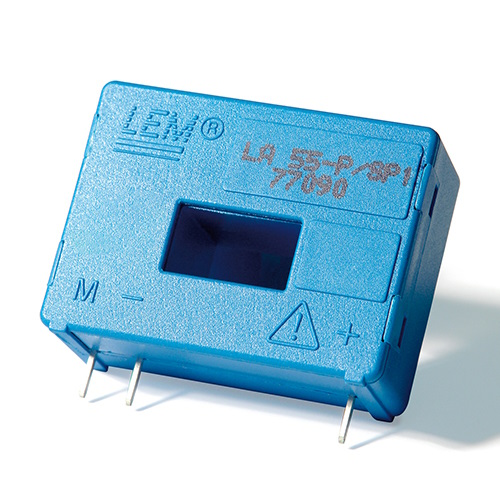
\includegraphics[width=0.4\linewidth]{img//SensorCorriente/sensor.jpg}
    \caption{Sensor LA 55-P}
    \label{fig:sensor}
\end{figure}

Para realizar su función, se atraviesa el cable cuya corriente va a ser medida por la abertura cuadrada que posee el sensor, de esta manera, el dispositivo entrega una corriente que se transforma a voltaje con una resistencia (R3 en el esquemático) y se amplifica mediante un circuito de amplificadores operacionales entregando un voltaje a la salida de la PCB (designado como 'SalidaSensorCorriente'), y posteriormente, este voltaje se digitaliza en el módulo OPTO-22 para ser comunicado al computador que realiza el control.

\begin{figure}[H]
    \centering
    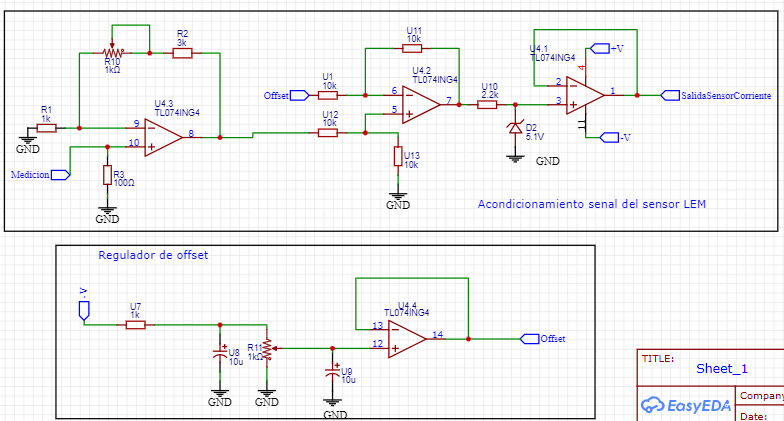
\includegraphics[width=0.75\linewidth]{img//SensorCorriente/sensorCorriente1.jpg}
    \caption{Acondicionamiento de la señal de corriente}
    \label{fig:sCorriente}
\end{figure}

Por ultimo, para realizar todas las funciones requeridas para acondicionar la señal de corriente, el circuito requiere de una fuente de alimentación simétrica como se ve en la fig. \ref{fig:fSimetrica}, el valor del voltaje de salida de la fuente es de +-12 Vdc.

\begin{figure}[H]
    \centering
    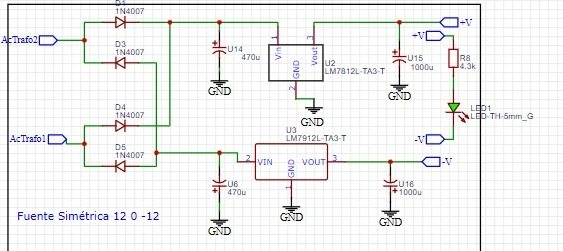
\includegraphics[width=0.75\linewidth]{img//SensorCorriente/fuenteSim.jpg}
    \caption{Fuente simétrica}
    \label{fig:fSimetrica}
\end{figure}

Cabe destacar que este módulo se alimenta gracias a un transformador simétrico de 12 Voltios RMS con un tap central, es decir, posee 3 cables de salida. Esto permite alimentar todas las PCB implementadas directamente desde la toma de 220 Voltios AC.

